\cleardoublepage
\chapter{Pelaksanaan Pekerjaan Bulan Juli}
\label{chap:judul-pekerjaan}
\makeatletter
\@addtoreset{figure}{section}
\makeatother
\renewcommand{\thefigure}{\thesection.\arabic{figure}}

\section{Gambaran Umum Pekerjaan}
Pada Juli 2026, penulis melaksanakan kerja praktik di PT Nutech Integrasi pada Divisi \textit{Business \& Product Development} sebagai \textit{Product Specialist Intern}. Kegiatan pada bulan pertama diawali dengan pengenalan pilar perusahaan dan mempelajari dokumen katalog produk PT Nutech Integrasi. Setelah memperoleh gambaran mengenai solusi perusahaan, penulis membantu mentor dalam eksplorasi awal \textit{Smart Depot Management System} (SDMS), khususnya informasi aset yang divisualisasikan dalam bentuk sistem antarmuka pemantauan.

Kegiatan ini mendorong penulis mengembangkan prototipe antarmuka web \textit{Operational Dashboard} sebagai fokus pekerjaan untuk bulan Juli. Rancangan dibuat secara mandiri oleh penulis dengan menggunakan hasil eksplorasi dalam menentukan kebutuhan informasi dan merancang penyajian informasi operasional depo. Secara keseluruhan, pekerjaan dilaksanakan melalui beberapa tahapan, mulai dari pemahaman penugasan, pendalaman informasi inspeksi, identifikasi kebutuhan tampilan, hingga pengembangan prototipe dashboard. Alur pelaksanaan pekerjaan tersebut ditunjukkan pada Gambar \ref{fig:alur-pekerjaan-juli}.

\begin{figure}[ht]
    \centering
    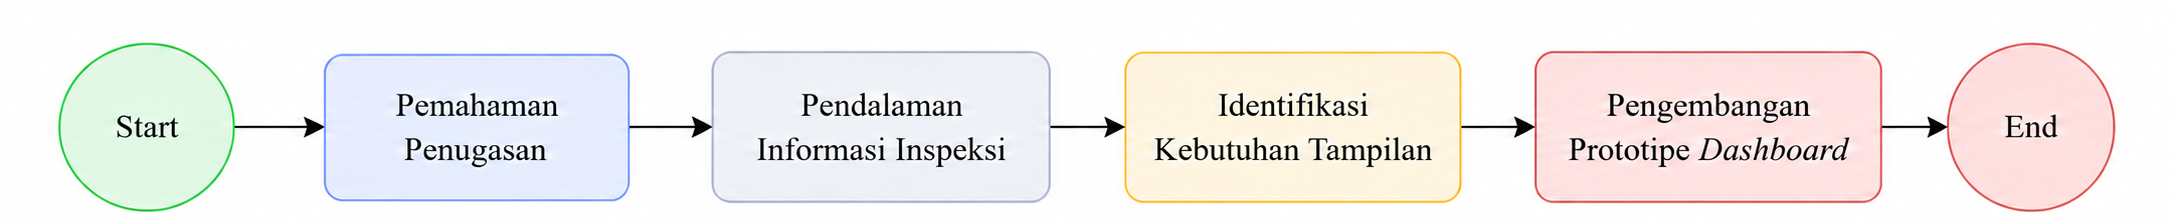
\includegraphics[width=0.8\textwidth]{images/JULI(2).png}
    \caption{Alur pelaksanaan pekerjaan bulan Juli}
    \label{fig:alur-pekerjaan-juli}
\end{figure}

\section{Pengenalan Portofolio dan Penyelarasan Dokumen Katalog Produk}
\subsection{Pengenalan Portofolio Perusahaan}
Fase awal kerja praktik adalah mempelajari portofolio produk dan solusi teknologi PT Nutech Integrasi. Hal ini penting dilakukan untuk memberikan pemahaman mengenai cakupan bisnis PT Nutech Integrasi dan memahami Divisi \textit{Business \& Product Development} secara lebih jauh. Pada tahap ini, penulis mempelajari empat pilar bisnis perusahaan yang dibagi dalam dua kelompok layanan. Kelompok \textit{Intelligent Mobility} terdiri atas \textit{Intelligent Transportation System} (ITS) dan \textit{Intelligent Logistic System} (ILS), sedangkan kelompok \textit{Intelligent Services} tersusun atas \textit{Intelligent Information System} (IIS) dan \textit{Geographic Information System} (GIS).

\subsection{Penyelarasan Dokumen Katalog Produk}
Dalam rangka mengoptimalkan proses pengelolaan data produk yang komprehensif, penulis melaksanakan serangkaian aktivitas verifikasi dan penyesuaian terhadap dokumen katalog yang dimiliki oleh PT Nutech Integrasi. Tujuan utama kegiatan ini adalah memastikan seluruh konten yang tercantum dalam katalog selaras dan merefleksikan secara akurat keempat pilar fundamental yang menopang strategi bisnis perusahaan. Kegiatan ini secara spesifik meliputi perbaikan substansial pada aspek penulisan. Selain itu, penulis juga melakukan pemeriksaan menyeluruh terhadap kelengkapan informasi, seperti Tingkat Komponen Dalam Negeri (TKDN) yang menunjukkan proporsi komponen dalam negeri, Klasifikasi Baku Lapangan Usaha Indonesia (KBLI) sebagai penanda sektor industri, Nomor Induk Berusaha (NIB) sebagai identitas legalitas bisnis, serta informasi mengenai hak cipta dan lisensi yang menyertai setiap produk.

\section{Kebutuhan Smart Depot Management System}
\subsection{Identifikasi Ruang Lingkup Smart Depot}
Setelah penyesuaian katalog produk dilakukan, penulis ditugaskan oleh mentor untuk mempelajari konsep \textit{Smart Depot Management System} (SDMS). Kegiatan ini diawali dengan memahami tujuan, ruang lingkup, dan penerapan SDMS dalam menawarkan solusi kepada sarana perkeretaapian Indonesia. Hal ini dilakukan melalui diskusi bersama mentor dan pencarian informasi pendukung dari negara-negara Eropa.

Eksplorasi difokuskan pada pemantauan kondisi komponen \textit{pantograph} dan \textit{wheelset}. Penulis mempelajari kebutuhan informasi pemeriksaan, seperti identitas aset, status kondisi, hasil inspeksi, riwayat pemeriksaan, dan indikator peringatan. Hasil pembelajaran ini digunakan sebagai pedoman awal dalam menetapkan informasi yang disajikan pada prototipe \textit{Operational Dashboard} berbasis web.

\subsection{Pantograph dan Wheel Inspection}
Dalam memahami kebutuhan pemantauan kondisi sarana perkeretaapian, penulis melakukan riset awal mengenai \textit{Pantograph Inspection} dan \textit{Wheel Inspection} melalui referensi yang berkaitan dengan pengembangan konsep \textit{Smart Depot Management System} (SDMS). Kegiatan ini penting untuk mengenali pemeriksaan yang diperlukan dalam pemantauan kondisi aset di depo. Pada \textit{Pantograph Inspection}, pembahasan berfokus pada kondisi pantograf, khususnya mengenai \textit{carbon strip}, termasuk petunjuk yang dipakai dalam pengujian. Sementara itu, eksplorasi \textit{Wheel Inspection} meliputi hasil pengukuran dan parameter kondisi roda sebagai dasar dalam pemantauan sarana.

Selanjutnya, penulis mempelajari proses pemeriksaan pantograf, teknologi yang digunakan, serta informasi yang dibutuhkan untuk memantau kondisi komponen tersebut. Hasil pembelajaran kemudian dirangkum ke dalam kerangka eksplorasi yang meliputi aspek operasional, komponen pemeriksaan, alternatif teknologi, dan kebutuhan pengguna. Kerangka ini digunakan sebagai referensi awal dalam pengembangan konsep \textit{Operational Dashboard}, sebagaimana ditunjukkan pada Gambar \ref{fig:kerangka-pantograph}.

\begin{figure}[ht]
    \centering
    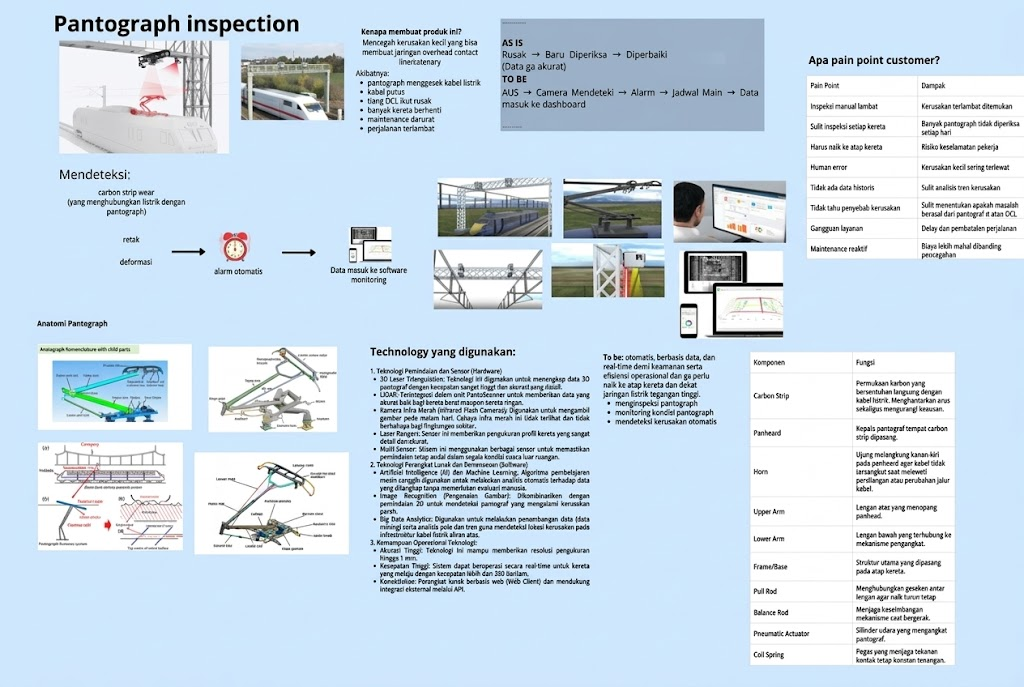
\includegraphics[width=0.72\textwidth]{images/kerangka.jpg}
    \captionsetup{justification=centering}
    \caption{Kerangka Eksplorasi Pantograph Inspection dan Identifikasi Kebutuhan Informasi}
    \label{fig:kerangka-pantograph}
\end{figure}

\subsection{Identifikasi Kebutuhan \textit{Operational Dashboard}}
Bagian dari proses pengembangan konsep \textit{Operational Dashboard} adalah melakukan identifikasi kebutuhan informasi. Proses ini bertujuan untuk menentukan jenis informasi yang disajikan dalam \textit{interface} pemantauan. Dalam tahap ini, penulis mengkaji informasi yang telah diperoleh mengenai pemeriksaan \textit{pantograph} dan \textit{wheelset}, kemudian menghubungkannya dengan kebutuhan pemantauan aset di lingkungan depo. Proses ini dilakukan dengan mempertimbangkan informasi yang dibutuhkan untuk mengetahui kondisi aset secara umum, memantau pelaksanaan inspeksi, serta mengidentifikasi hasil pemeriksaan komponen yang rusak atau perlu segera ditangani.

Untuk menyusun antarmuka tersebut, penulis membagi kelompok kebutuhan informasi ke dalam tujuh bagian utama, yaitu \textit{Overall Asset Status}, \textit{Inspection Status}, \textit{Pantograph Result}, \textit{Wheel Result}, \textit{Active Alarm}, \textit{History/Trend}, dan \textit{Recommendation/Action}. Masing-masing komponen memiliki peran yang berbeda dalam menampilkan informasi kondisi aset dan aktivitas inspeksi. Pengelompokan ini dilakukan agar informasi yang bersifat umum dapat dibedakan dari hasil pemeriksaan yang lebih spesifik, sehingga susunan dashboard dapat dirancang secara terstruktur dan mudah dipahami. Rincian komponen beserta tujuan penyajiannya ditunjukkan pada Tabel \ref{tab:pengelompokan-dashboard}.

\begin{table}[ht]
    \centering
    \caption{Pengelompokan \textit{Operational Dashboard}}
    \label{tab:pengelompokan-dashboard}
    \begin{tabularx}{0.9\textwidth}{|>{\raggedright\arraybackslash}X|>{\raggedright\arraybackslash}X|}
        \hline
        \textbf{Komponen} & \textbf{Tujuan penyajian dalam rancangan} \\
        \hline
        \textit{Overall Asset Status} & Ringkasan kondisi aset \\
        \hline
        \textit{Inspection Status} & Status pelaksanaan inspeksi \\
        \hline
        \textit{Pantograph Result} & Kelompok hasil pemeriksaan pantograf \\
        \hline
        \textit{Wheel Result} & Kelompok hasil pemeriksaan roda \\
        \hline
        \textit{Active Alarm} & Indikasi masalah \\
        \hline
        \textit{History/Trend} & Menyediakan area visualisasi perubahan kondisi \\
        \hline
        \textit{Recommendation/Action} & Menyediakan area informasi \\
        \hline
    \end{tabularx}
\end{table}

\section{Proses Perancangan \textit{Operational Dashboard}}
\subsection{Penyusunan Konsep Dashboard}
Fase utama dalam perancangan \textit{Operational Dashboard} adalah memastikan fokus penyampaian informasi sesuai dengan kebutuhan yang telah diidentifikasi pada tahap eksplorasi sebelumnya. Penulis berfokus pada penyusunan tampilan yang memberikan gambaran umum mengenai kondisi aset dan aktivitas inspeksi di lingkungan depo. Informasi yang bersifat ringkasan, seperti \textit{Overall Asset Status} dan \textit{Inspection Status}, diprioritaskan sebagai bagian utama agar pengguna dapat memahami gambaran awal mengenai kondisi operasional tanpa harus memeriksa setiap hasil inspeksi secara manual.

Selain informasi ringkasan, penulis menyajikan hasil \textit{Pantograph Inspection} dan \textit{Wheel Inspection} dalam kelompok tampilan yang berbeda agar kondisi setiap aspek dapat dikenali dengan cepat dan jelas. Informasi tambahan seperti \textit{Active Alarm}, \textit{History/Trend}, dan \textit{Recommendation/Action} menjadi faktor pendukung untuk melengkapi tampilan visual peringatan, riwayat kondisi aset, serta kebutuhan observasi lanjutan.

\subsection{Implementasi Antarmuka Tahap Awal}
Dalam mengembangkan antarmuka web, penulis menggunakan HTML (\textit{HyperText Markup Language}), CSS (\textit{Cascading Style Sheets}), dan JavaScript untuk menyusun struktur halaman serta mengarahkan elemen dashboard agar selaras dengan kebutuhan. CSS digunakan untuk mengatur tata letak, ukuran komponen, warna, dan kejelasan informasi supaya tampilan dashboard tersusun secara konsisten. Sementara itu, JavaScript digunakan untuk membangun pola interaksi pengguna dengan prototipe agar dapat digunakan secara lebih intuitif dan nyaman.

Penerapan teknologi juga membantu penyusunan tampilan visual dan perilaku antarmuka secara lebih terstruktur. Proses pengembangan berfokus pada penyusunan antarmuka yang menampilkan ringkasan kondisi aset, status inspeksi, hasil pemeriksaan pantograf dan roda secara terintegrasi, serta informasi pendukung dalam satu halaman. Hasil kegiatan ini berupa prototipe web yang berfungsi sebagai pedoman awal untuk menggambarkan konsep operasional depo, meskipun pengembangannya masih terbatas pada fungsionalitas antarmuka dan interaktivitas dasar.

\subsection{Penyusunan Komponen Dashboard}
Proses pengembangan dilakukan dengan menyusun komponen \textit{Operational Dashboard} dari modul yang telah diidentifikasi sebelumnya. Pada tahap ini, penulis mengatur susunan elemen antarmuka agar setiap informasi memiliki bagian tampilan yang sesuai dengan fungsinya. Komponen \textit{Overall Asset Status} dan \textit{Inspection Status} ditempatkan sebagai bagian ringkasan untuk memberikan gambaran umum mengenai kondisi aset dan aktivitas inspeksi di lingkungan depo.

Selanjutnya, hasil \textit{Pantograph Inspection} dan \textit{Wheel Inspection} disusun dalam komponen terpisah agar informasi kondisi masing-masing aset dapat dibedakan dengan jelas. Komponen pendukung, seperti \textit{Active Alarm}, \textit{History/Trend}, dan \textit{Recommendation/Action}, juga digunakan untuk menampilkan peringatan, riwayat kondisi, serta informasi mengenai tahapan pemeriksaan lanjutan.

\subsection{Pengaturan Tata Letak dan Interaksi Antarmuka}
Pada tahap ini, pengembangan prototipe \textit{Operational Dashboard} dilakukan dengan menata tata letak dan interaksi antarmuka agar informasi dapat disajikan secara jelas dan mudah dipahami. Proses pengembangan pada tahap ini meliputi penyusunan tata letak komponen, pengaturan tampilan visual, serta penerapan interaksi dasar pada dashboard. Kegiatan yang dilakukan meliputi:

\begin{enumerate}[a.]
    \item \textbf{Penataan tata letak komponen}, meliputi penempatan kartu informasi, ukuran komponen, dan jarak antarelemen agar dashboard terlihat rapi.
    \item \textbf{Penataan tampilan visual}, meliputi penggunaan warna, tipografi, serta gaya tampilan untuk membedakan setiap kelompok informasi.
    \item \textbf{Peningkatan dinamika antarmuka}, mencakup penerapan prinsip dasar interaksi dengan memanfaatkan JavaScript.
\end{enumerate}

\subsection{Batasan Pengembangan}
Sampai tahap ini, pengembangan \textit{Operational Dashboard} masih berada dalam lingkup prototipe antarmuka berbasis web. Walaupun dalam pengerjaan proyek ini penulis telah menggunakan HTML, CSS, dan JavaScript, prototipe yang dihasilkan belum dikembangkan sebagai aplikasi operasional yang terintegrasi dengan perangkat inspeksi maupun sistem pengelolaan data depo.

\section{Hasil Pekerjaan dan Pembelajaran}
Selama pelaksanaan kerja praktik pada bulan Juli, penulis memperoleh pengalaman dalam memahami portofolio produk perusahaan, melakukan pemeriksaan dokumen katalog, serta mengeksplorasi kebutuhan informasi dalam pengembangan konsep \textit{Smart Depot Management System} (SDMS). Salah satu hasil pekerjaan yang dikembangkan adalah prototipe \textit{Operational Dashboard} berbasis web yang menampilkan gambaran awal mengenai pemantauan kondisi aset dan aktivitas inspeksi di lingkungan depo.
